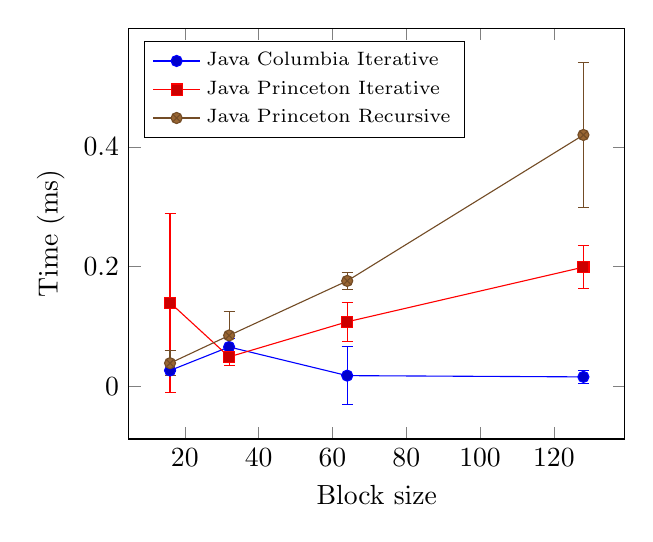
\begin{tikzpicture}
\begin{axis}[xlabel={Block size},ylabel={Time (ms)},width=0.65\linewidth,legend pos=north west,scaled y ticks = false,legend cell align=left,legend style={font=\scriptsize}]
\addplot+[error bars/.cd, y dir=both,y explicit] coordinates {
(16, 0.0265) +- (0.0011, 0.0011)
(32, 0.0658) +- (0.0148, 0.0148)
(64, 0.0179) +- (0.0486, 0.0486)
(128, 0.0158) +- (0.0105, 0.0105)
};
\addplot+[error bars/.cd, y dir=both,y explicit] coordinates {
(16, 0.1398) +- (0.1496, 0.1496)
(32, 0.0492) +- (0.0139, 0.0139)
(64, 0.1078) +- (0.0326, 0.0326)
(128, 0.1991) +- (0.0359, 0.0359)
};
\addplot+[error bars/.cd, y dir=both,y explicit] coordinates {
(16, 0.0387) +- (0.0210, 0.0210)
(32, 0.0850) +- (0.0396, 0.0396)
(64, 0.1761) +- (0.0136, 0.0136)
(128, 0.4199) +- (0.1211, 0.1211)
};
\legend{Java Columbia Iterative , Java Princeton Iterative , Java Princeton Recursive}
\end{axis}
\end{tikzpicture}
